\fig{fv:h3:paths}{经过同一初态的不同路径，具有不同斜率与曲线下面积}{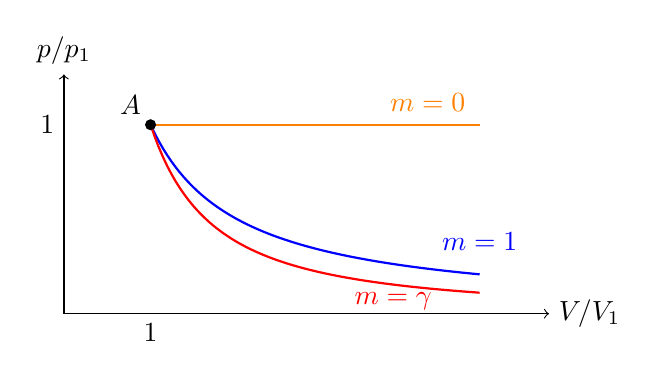
\begin{tikzpicture}[x=1.1cm,y=.8cm]
\draw[->](0,0)--(5.6,0)node[right]{$V/V_1$};\draw[->](0,0)--(0,3.8)node[above]{$p/p_1$};
\draw[blue,thick,domain=1:4.8,samples=80]plot(\x,{3/\x});\draw[red,thick,domain=1:4.8,samples=80]plot(\x,{3/pow(\x,1.4)});
\draw[orange,thick](1,3)--(4.8,3);\fill(1,3)circle(2pt)node[above left]{$A$};\node[left]at(0,3){$1$};\node[below]at(1,0){$1$};
\node[orange]at(4.2,3.35){$m=0$};\node[blue]at(4.8,1.15){$m=1$};\node[red]at(3.8,.2){$m=\gamma$};\end{tikzpicture}}
图\ref{fv:h3:paths}中的 $m$指多方指数，$pV^m=\text{常量}$给局部斜率 $\dd p/\dd V=-mp/V$。从同一状态膨胀，绝热线比等温线下降更快，因而到相同体积时温度更低、对外功也更小。路径方程只把状态变量联系起来；热量仍须由 $Q=\Delta U+\int p\dd V$另算。尤其 $m=1$的积分是对数，不能直接代入含 $1-m$分母的普通幂积分式。
